\documentclass{standalone}
\usepackage{pgfplots}
\pgfplotsset{compat=1.18}

\begin{document}

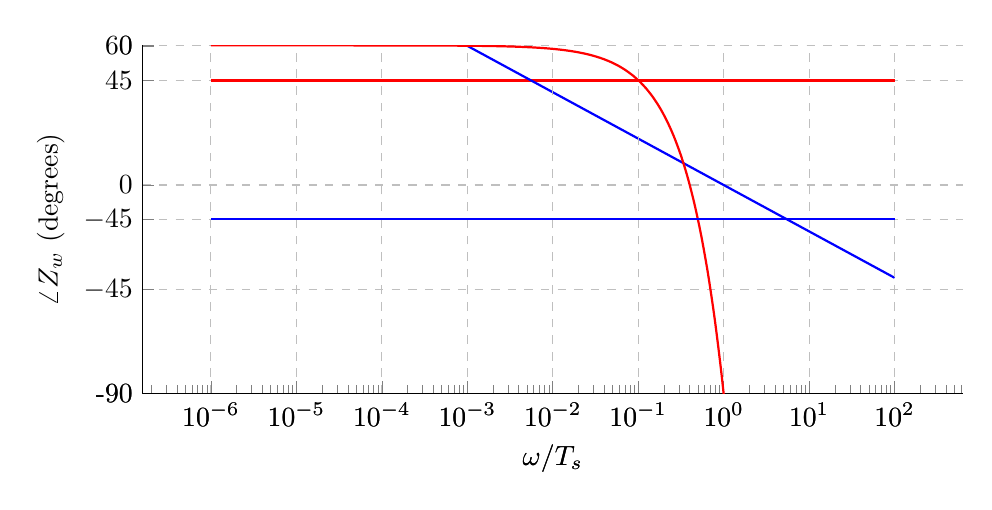
\begin{tikzpicture}
    \begin{semilogxaxis}[
        title={},
        xlabel={$\omega/T_s$},
        ylabel={},
        ymin=-90, ymax=60,
        ytick={-90,-45,0,45,60},
        yticklabels={-90,$-45$,0,45,60},
        ylabel near ticks,
        axis x line*=bottom,
        axis y line*=left,
        legend style={at={(0.03,0.03)},anchor=south west},
        grid=major,
        grid style=dashed,
        width=12cm,
        height=6cm,
        every axis plot/.append style={
            thick,
            mark=none,
            domain=1e-6:1e2,
            samples=100,
            smooth
        }
    ]
        \addplot [red] {45};
        \addplot [blue] {-20*log10(x)};
    \end{semilogxaxis}

    \begin{semilogxaxis}[
        title={},
        xlabel={$\omega/T_s$},
        ylabel={$\angle Z_w$ (degrees)},
        ymin=-90, ymax=0,
        ytick={-90,-45,0},
        yticklabels={-90,$-45$,0},
        ylabel near ticks,
        axis x line*=bottom,
        axis y line*=left,
        legend style={at={(0.03,0.03)},anchor=south west},
        grid=major,
        grid style=dashed,
        width=12cm,
        height=6cm,
        every axis plot/.append style={
            thick,
            mark=none,
            domain=1e-6:1e2,
            samples=100,
            smooth
        }
    ]
        \addplot [red] {-90*x};
        \addplot [blue] {-45};
    \end{semilogxaxis}
\end{tikzpicture}

\end{document}